\subsection{Data Structures}
The data structures used within the \textit{TravelGood} RESTful and SOAP/BPEL are depicted in figure \ref{classdiagramBPEL} and figure \ref{classdiagramREST}. Although describing the exact same process, the two implementations of \textit{TravelGood} are different and therefore use somewhat different data structures. More details about what are the main differences follow in the discussion below. 

\begin{figure}[H]
\centering
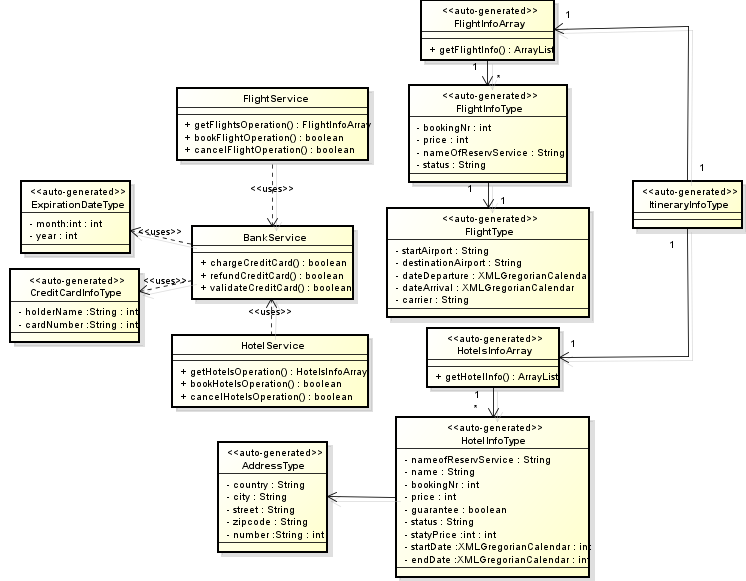
\includegraphics[width=0.9\textwidth]{images/BPEL-SOAP}
\caption{Class diagram of \textit{TravelGood} BPEL/SOAP.}
\label{classdiagramBPEL}
\end{figure}

\textit{Itinerary} (ItineraryInfoType) is the main data object that will be manipulated by \textit{TravelGood} operations. It contains two arrays of \textit{FlightInfo} (\textit{FlightInfoType}) and \textit{HotelInfo} (\textit{HotelInfoType}) data objects that will be populated by the user during the planning phase when calling the \textit{addFlightToItinerary()} and \textit{addHotelToItinerary()} operations. Although the \textit{FlightInfo} and \textit{FlightInfoType} classes contain the same attributes (as is the case for \textit{HotelInfo} and \textit{HotelInfoType}), different data structures are created separately for both REST and SOAP/BPEL services since the first one requires classes to be annotated with \textit{\@ XMLRootElement} whereas the latter works with auto-generated classes from the WSDL complex types declarations. Same principle applies for the \textit{CreditCard} (\textit{CreditCardInfoType}) data object required for communication with \textit{FastMoney} web service.

\begin{figure}[H]
\centering
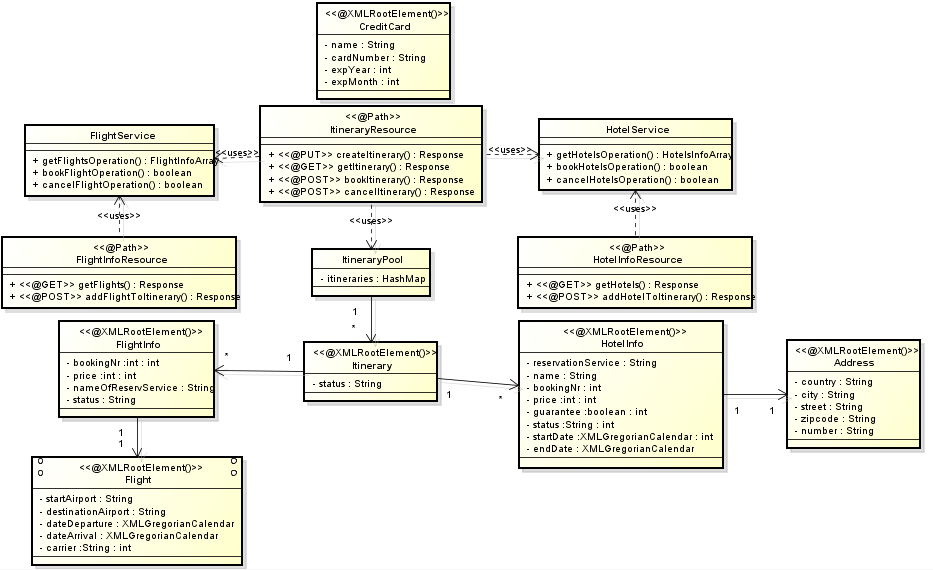
\includegraphics[width=\textwidth]{images/REST}
\caption{Class diagram of \textit{TravelGood} REST.}
\label{classdiagramREST}
\end{figure}

Information about flights and hotels is stored, maintained and manipulated by the external web services, \textit{LameDuck} and \textit{NiceView}. Therefore, when calling their operations, both implementations of \textit{TravelGood}’s operations need to make sure that the right input types are used. In BPEL, this consistency is easily ensured by having and XML Schema Document enclosing the declaration of all complex types necessary for \textit{LameDuck}, \textit{NiceView} and \textit{TravelGood}. In REST, however, this is not as straightforward since \textit{TravelGood} uses \textit{XMLRootElements} such as \textit{FlightInfo}, \textit{HotelInfo}, \textit{CreditCard} which need to be transformed to \textit{FlightInfoType}, \textit{HotelInfoType} and \textit{CreditCardType} in order to be understood by the external web services. This transformations are ensured inside the \textit{FlightService} and \textit{HotelService} classes (see figure \ref{classdiagramREST}).

In addition, inside \textit{LameDuck} and \textit{NiceView} services, each flight and hotel data is represented with \textit{Flight} (\textit{FlightType}) and \textit{Hotel} (\textit{HotelType}) classes where their instances contain static data (name, address, start airport, destination, etc.) of the entity they are representing. When a user requests a flight information, we create the instances of classes \textit{FlightInfo} (\textit{FlightInfoType}) and \textit{HotelInfo} (\textit{HotelInfoType}) that contain additional information (such as booking number, price, status) on top of \textit{Flight} and \textit{Hotel}. With these additional information, the flight or hotel can be booked and the bookings can be tracked. 

Last but not least, REST uses resources (\textit{\@ Path}) on top of all the data objects discussed above which can be accessed by the user via URLs in order to execute different operations (create, book, cancel, etc). This is not the case in BPEL, when only complex types are used for all client-WS or WS-WS interactions. This matter will be discussed more in-depth in the following sections.
